\subsection{UC13 - Creazione prodotto}
\begin{figure}[H]
  \centering
  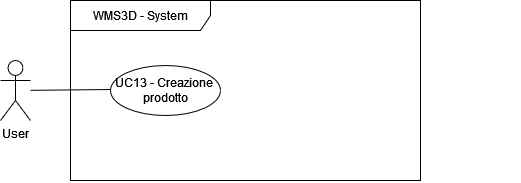
\includegraphics[width=0.8\textwidth]{UC_diagrams_11-20/UC13_sys.drawio.png}
   \caption{Diagramma UML UC13 - Creazione prodotto}
\end{figure}
\begin{figure}[H]
  \centering
  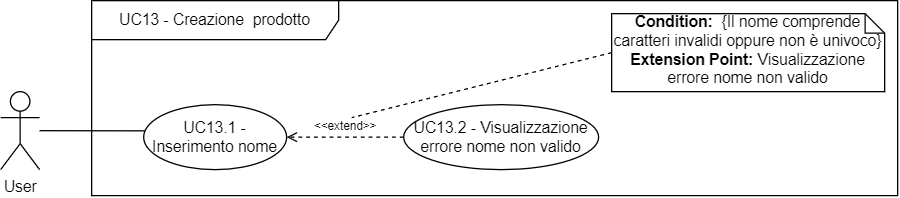
\includegraphics[width=0.8\textwidth]{UC_diagrams_11-20/UC13.drawio.png}
   \caption{Diagramma UML in dettaglio UC13 - Creazione prodotto}
\end{figure}
\begin{itemize}
    \item \textbf{Attori:} User.
    \item \textbf{Pre-condizione:}  L'utente ha creato/caricato un magazzino [UC1].
    \item \textbf{Post-condizione:} L'utente crea un prodotto che viene aggiunto in libreria.
    \item \textbf{Scenario Principale:}  L'utente crea un prodotto, inserendo un nome univoco [UC13.1].
    \item \textbf{Generalizzazioni:} -
    \item \textbf{Estensioni:} -
\end{itemize}


\subsubsection{UC13.1 - Inserimento nome}
\begin{itemize}
    \item \textbf{Attori:} User.
    \item \textbf{Pre-condizione:}  L'utente ha creato/caricato un magazzino [UC1] e vuole creare un prodotto.
    \item \textbf{Post-condizione:} L'utente ha dato un nome identificativo al nuovo prodotto.
    \item \textbf{Scenario Principale:}  L'utente inserisce un nome univoco per il nuovo prodotto.
    \item \textbf{Generalizzazioni:} -
    \item \textbf{Estensioni:} È presente una estensione:
    \begin{itemize}
        \item UC13.2 - Visualizzazione errore nome non valido.
    \end{itemize}
\end{itemize}


\subsubsection{UC13.2 - Visualizzazione errore nome non valido}
\begin{itemize}
    \item \textbf{Attori:} User.
    \item \textbf{Pre-condizione:}  L'utente ha inserito un nome identificativo di un prodotto che contiene caratteri invalidi oppure non è univoco.
    \item \textbf{Post-condizione:}  L'utente visualizza un messaggio d'errore e dovrà reinserire un nome diverso.
    \item \textbf{Scenario Principale:}  L'utente visualizza un messaggio informativo sull'errore e ne conferma la ricezione. L'operazione fallisce e l'utente dovrà scegliere un nuovo nome.
    \item \textbf{Generalizzazioni:} -
    \item \textbf{Estensioni:} -
\end{itemize}